\chapter{Protocol Design and Encoding}
% – Describe the design of what you have created.
% – Start with the application architecture, giving its overall structure
% and the components that make up that structure.
% – Give a description of the design of each of the the components that
% make up the architecture.
% – Include the database or storage representation.
% – Provide implementation details as necessary.

This chapter has been split into two parts. First is the `Modelling'
section where look at the design of the adapted protocol and the state
transitions for Paxos. We also look at the Python simulator
that helped solidify these designs before encoding them in Disel.
The latter part of this chapter explains how the adapted protocol was
encoded in Disel.

\section{Modelling}

\subsection{The Adapted Protocol}
For mechanising the proof of Paxos in Disel, we followed the approach highlighted
in the Disel section of Chapter 3. Applying this approach meant
we needed to come up with the state transition system and the inductive invariant
for the protocol which we will encode in Disel. Before coming up with these things
though, we decided to simplify the actual simple Paxos protocol that we will prove.

The goal of this simplification was to reduce the amount of things that we will need
to prove in Disel by focusing on the `core' parts of the protocol which
lead to consensus being achieved. The `convenience' parts of the protocol, like
the sub phase of informing the learner, aren't necessary for consensus being
achieved in the global state and can also be proved separately after we have
finished proving the `core' parts of the protocol. Garcia-Perez et al \cite{6}
have also showed how the optimizations of a protocol can be verified separately
from the `core' protocol. In their paper, they produce a verified implementation
of multi Paxos using their verified implementation of simple Paxos.

In order to adapt the protocol and focus on the `core' parts, the first thing
we did was to do away with the `Informing the learner' phase of simple Paxos.
This is the phase where once an acceptor has accepted a proposal, it then informs
a leaner by sending it an accepted request. We decided against proving this
because we can use the inductive invariant to check the global state of the system.
The inductive invariant allows to check when a majority of acceptors have
accepted a proposal and what proposal each of them has accepted. Thus, we can know
from the inductive invariant when consensus has been achieved by checking the values
of each of the accepted proposals.

Getting rid of the learning phase also meant that we did not have to implement
a learner.
% in our protocol as the role of the learner (detecting that consensus
% has been achieved) is performed by the inductive invariant.
The learner is useful in the actual Paxos implementations as
it can detect when consensus is achieved and can then inform the client, yet, its
presence does not change how consensus is achieved. Removing the learner simplified
our state transition diagram for the protocol as we did not have to account
for the states of the learner and also the $Phase 2b$ transition of the
accepted request.

Additionally, we decided to remove some optimisations from the protocol.
Optimisations are aspects of the protocol that improve its running time or
resource consumption by improving upon the `mundane' way of doing the same
thing. Removing optimisations allowed us to simplify our proofs in Disel.

Therefore, we decided that if a proposer fails while trying to achieve
consensus with a proposal number (i.e. it receives a nack), then it does not later try
to propose again with a higher proposal number. Removing this optimisation meant we did not
have to deal with the state of a proposer where it changes the proposal number it
was initialised with. Removing this optimisation only
effects the liveness of the protocol but not its safety, as if a proposer
receives a nack, it is just an indication that it will not be able to achieve
consensus with the proposal number that it is currently using. Thus, in order
for consensus to be achieved, a proposer which is initialised with a higher
proposal number will have to successfully get promises from a quorum of acceptors.

% Additionally we removed the minor optimisation of choosing a majority for
% sending requests from the proposer. The proposer instead of choosing a
% quorum of acceptors for sending a message, chooses the entire set of acceptors.
% This does not alter the protocol as the entire set of acceptors is a valid
% quorum of acceptors.

This adapted and simplified protocol allows us to focus on verifying the core
logic (the part dealing with achieving consensus) of Paxos. The
optimisations and `convenience' that we removed can be verified separately after
the core logic has been verified.


\subsection{State Transitions}
Having adapted the protocol, we then had to create a state transition system for
the nodes in our protocol in order to encode it in Disel. For creating the states,
we need to look at what the function of each node is in the protocol at a particular
moment and what type of data it holds at that time.

A node should only be able to transition from one state to another when it either
receives or sends a message. Therefore, the data held by the node in each state
should be enough for it to be able to create the message it wants to send or to
be able to correctly process the message it receives.

We tried to minimise the number of states and transitions between them, in order
to simplify the proof in Disel. This was important because each state transition
has to be shown to hold with the invariant so reducing the state transitions,
reduces the number of proofs.

We decided that a node can either be initialised as an acceptor or a proposer.
The state transitions of each node will depend upon this initial state, so below
we will separately look at the state transition systems for the proposer and the
acceptor.

The main difference between the state transition for the acceptor and the proposer
is that the acceptor sends and receives messages from a single proposer while a
proposer has to send and receive messages from all the acceptors.


\subsubsection{Proposer}
\begin{figure}
\centering
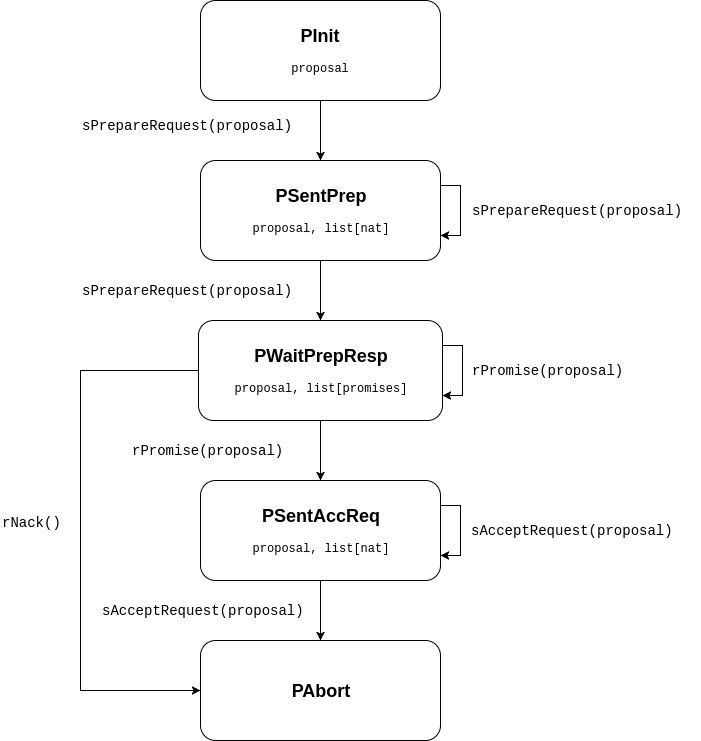
\includegraphics[width=\textwidth]{figures/proposer_state_transitions.png}
\caption{Proposer State Transition Diagram
\label{fig:myInlineFigure}}
\end{figure}

The proposer starts off in the \texttt{PInit} state where it is initialised with
a \texttt{proposal} (a custom defined data type which is tuple of two natural numbers),
$\langle p, v \rangle$.
The natural number $p$ is the proposal number and $v$ is the value that the
proposer tries to achieve consensus on. This means that the first prepare
request this proposer sends will include this proposal $\langle p, v \rangle$.

The proposer then moves to the \texttt{PSentPrep} state when it starts to send prepare
requests to the acceptors. In this state, the proposer still holds the proposal
but additionally now also stores a list of natural numbers, \texttt{sent\_to}. This list stores the
natural number identifiers of the acceptors, this proposer has sent requests to.
Whenever it sends a prepare request to an acceptor, it adds the identifier of
the acceptor to this list.
The proposer remains in the \texttt{PSentPrep} state and keeps sending prepare requests
until the contents of \texttt{sent\_to} become equal to the global list \texttt{acceptors} which
holds the identifiers of all the acceptors in the system. This means the proposer
stays in this state until it has sent a prepare request to every single acceptor
in the system.

Once the proposer has sent the last prepare request, it them transitions to
the \texttt{PWaitPrepResp} state. In this state the proposer again holds a proposal and
another list \texttt{promises} which is defined as below to be a list of tuples
each containing a \texttt{nid} (a natural number identifier for a node), a boolean
and a \texttt{proposal}.

\begin{lstlisting}
Definition promises := seq (nid * bool * proposal).
\end{lstlisting}

The proposer stays in this state and keeps receiving messages from the acceptor
until one of the following two things happen:
\begin{enumerate}
  \item It receives a nack response from the acceptor. This indicates that the
    acceptor might already have promised a proposal
    with a proposal number greater than $p$. This makes the proposer
    transition into the \texttt{PAbort} state. In this state the proposer basically
    gives up trying to achieve consensus using the proposal number $p$ that it was
    initialised with and completely stops sending and receiving messages. Hence,
    the proposer doesn't need to hold any data in this state.
  \item It receives a promise response from every single acceptor. When this
    happens, the proposer transitions to the \texttt{PSentAccReq} state.
\end{enumerate}

When the proposer reaches the \texttt{PSentAccReq}, it means it has received a promise
from every single acceptor and it can now start sending accept requests to each
of the acceptors in the system. In the \texttt{PSentAccReq} the proposer again stores
a list \texttt{sent\_to} to keep track of every single acceptor it has already sent the
accept request to. It also stores another \texttt{proposal} which is has the same
proposal number $p$ that the proposer was initialised with but the value $v$ is the
the value from the highest numbered proposal it received in a promise response.
In the verification section, we will look at how it determines this value by looping over
the \texttt{promises} list from the \texttt{PWaitPrepResp} state. The sending of
accept requests works similar to sending prepare requests in the
\texttt{PSentPrep} state. Finally, when the proposer finishes sending the
accept requests to all the acceptors, it transitions to the \texttt{PAbort}
state where it stops sending and receiving messages.


\subsubsection{Acceptor}
\begin{figure}
\centering
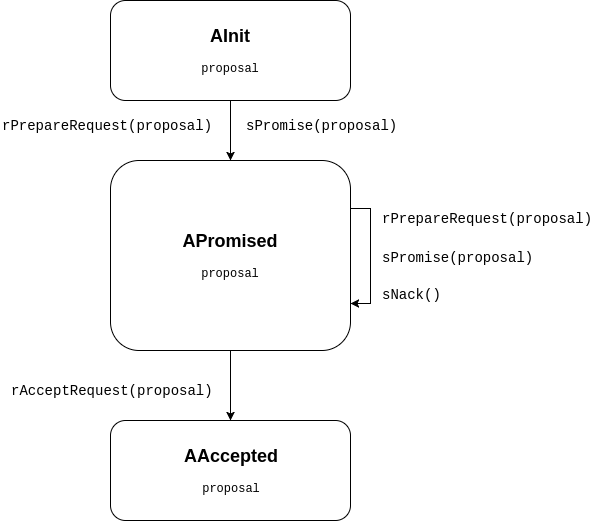
\includegraphics[width=0.7\textwidth]{figures/acceptor_state_transitions.png}
\caption{Acceptor State Transition Diagram
\label{fig:myInlineFigure}}
\end{figure}

The acceptor starts off in the \texttt{AInit} state. It does not hold any data
in this state as it is not sending any messages. It keeps listening for messages
and on receiving a prepare request message, it transitions to \texttt{APromised}
state.

In the \texttt{APromised} state, the acceptor holds a proposal. This is
the highest numbered proposal that it has received so far in a prepare request
message. In this state, on receiving a prepare request, if the proposal number
of the proposal in the prepare request is greater than the proposal number of
the proposal it currently holds, it updates its current state to hold the new
proposal but still remains in the \texttt{APromised} state. If the proposal
number of the proposal in the prepare request is not greater, the acceptor
sends a nack response to the proposer who sent the prepare request and does not
update its state.

An acceptor in the \texttt{APromised} state, on receiving an accept request, if
the value of the proposal number of the proposal in the accept request is greater than
the proposal number of the proposal that it currently holds, it transitions to the
\texttt{AAccepted} state where it now holds the new proposal with the greater
proposal number. If the proposal number of the new proposal number is not greater,
the acceptor remains in the same state.

In the \texttt{AAccepted} state, the acceptor stops listening for and responding
to messages. This is similar to the \texttt{PAbort} state for the proposer.

% \subsection{Inductive Invariant}
% A critical part of proving our protocol in Disel was designing an inductive invariant
% for our adapted protocol. The inductive invariant helps ensure the correctness of
% our adapted protocol enabling us to imposing requirements on the global state of the system.
% For proving the correctness of Paxos we found that our invariant had to capture
% when consensus is achieved on a value and also that once consensus is achieved
% on a particular value, further rounds of the protocol don’t change this value.
%
% \begin{quote}
% Inductive invariant means a property which when it holds for a state $s$,
% it will hold for any state $s'$ reachable from $s$.
% \end{quote}
%
% The crux of Paxos' correctness lies in the prepare phase where, before sending
% the accept request, the proposer must first set the value of the proposal, that
% it wants to propose, to be the value of the highest numbered proposal it receives
% as a promise. This ensures that when consensus has been achieved on a value `v',
% further rounds of the protocol also ensure that consensus will only be achieved on `v'.
%
% We established two invariants \textbf{I1} and \textbf{I2} which together form an inductive
% invariant for our protocol that also proves its safety.
%
% \begin{itemize}
%   \item \textbf{I1} simply tries to say that there can only be one unique value
%     associated with a particular proposal number for any proposal that has been accepted.
%   \item \textbf{I2} states that once consensus has been achieved on a value v,
%     every higher number proposal accepted by an acceptor also has the value v.
% \end{itemize}
%
% The mathematical representations for the invariants is given by.
% \begin{itemize}
%   \item \textbf{I1} - $\forall a_i, a_j \in A, \langle p, v_i \rangle \in a_{i}.accepted
%   \land \langle p, v_j \rangle \in a_{j}.accepted \rightarrow v_i = v_j$.
%   \item \textbf{I2} - $\forall a \in A, \forall \langle p_i, v_i \rangle \in a.accepted
%     \rightarrow \forall \langle p_j, v_j \rangle \in  a.accepted \land p_j > p_i
%     \rightarrow v_j = v_i$.
% \end{itemize}
%
% \textbf{I1} is preserved because if there are n proposers, they are
% initialised with a unique proposal number and throughout the running of the
% adapted protocol, the proposer always uses this unique proposal number for any
% value that it proposes. Hence, two different proposers never propose a proposal
% with the same proposal number as they all are initialised with different
% proposal numbers. Additionally, each proposer only sends one round
% of accept requests with the same proposal. So as each proposer proposes only one
% value with a unique proposal number, hus, we can conclude that each accepted proposal
% will have a unique value associated with a particular proposal number.
%
% For proving that \textbf{I2} is preserved, we need to show that once consensus
% has been achieved
% on a proposal with value $v$ then every other proposal, with a higher
% proposal number, on which consensus is achieved will also have
% proposal value set to $v$.
%
% In order for consensus to be achieved on a new proposal, the new
% proposal first needs to be accepted by an acceptor.
% So we can reduce the requirement as follows.
%
% $\Rightarrow$ If consensus has been achieved on a proposal
% $\langle p_1, v_1 \rangle$ then every other proposal $\langle p_2, v_2 \rangle$
% accepted by any acceptor, where $p_2 > p_1$, has $v_2 = v_1$.
%
% Further, acceptors can only accept a proposal which has been proposed
% by a proposer.
%
% $\Rightarrow$ If consensus has been achieved on a proposal $\langle p_1, v_1 \rangle$
% then every accept request $\langle p_2, v_2 \rangle$ sent by the proposer with
% $p_2 > p_1$, has $v_2 = v_1$.
%
% \begin{equation}
% \textrm{In order to prove the above, let's assume that consensus has been
% achieved on a proposal} \langle p_1, v_1 \rangle.
% \end{equation}
%
% After that lets say that the systems achieves consensus on
% $\langle p_2, v_2 \rangle$ where $p_2 > p_1$ and there does not exist $p_x$ such
% that consensus has been achieved on a proposal with proposal
% number $p_x$ where $p_1 < p_x < p_2$.
%
% So from our assumption (4.1), there must be a majority of acceptors
% such that they have accepted the proposal $\langle p_2, v_2 \rangle$.
% So we need to show that in $v_2 = v_1$.
% This is ensured in Paxos because of Phase 1 where the proposer must first
% get promises from a majority.
%
% So any majority the proposer for $p_2, v_2$ gets in Phase 1,
% will have at least one acceptor $a$ that has accepted $\langle p_1, v_1 \rangle$.
% Paxos also ensures that before sending the accept request for
% $p_2, v_2$, the proposer must select the value of the highest numbered
% proposals which it receives in its promises.
%
% So the acceptor $a$ will send $\langle p_1, v_1 \rangle$ in its promise message to
% the proposer. As $\langle p_2, v_2 \rangle$ is the only proposal number which has
% proposal number greater than $p_1$, the proposer must set $v_2 = v_1$ in its
% accept request message $\langle p_2, v_2 \rangle$ as $v_1$ is the value of the
% highest numbered proposal that it receives as a promise response.
% Thus, meeting our above requirement.

\subsection{Simulator}
%% Talk about how it modelled how Disel works
%% and how it followed our adapted protocol
The next step after designing the adapted protocol was to
implemented a simulator for it in Python. The simulator was modelled according
to Disel in that, each process has send and receive transitions and that each
node follows a state transition system. In order to test the protocol, we only
used the state transitions we designed in the adapted protocol. The type
of messages that each node sends or receives and the data it holds
were all taken from the state transition system.

In the code listing below you can see the main body that an acceptor node
runs in the simulator. It first checks the type of message and then performs
an action depending on its current state. For example, when it receives a
\texttt{AcceptRequestMessage}, if it is in the \texttt{AInit} state then it
accepts the proposal, otherwise if it is in the \texttt{APromised} state, it
first checks the proposal number of the incoming message (proposal)
and accepts the proposal only if the number is greater than the number
the acceptor has promised already.

\begin{lstlisting}[language=Python]
class Acceptor(Process):
    ...
    def body(self):
        while True:
            msg = self.get_next_msg()
            p_no, p_val = msg.proposal

            if isinstance(msg, PrepareRequestMessage):
                if self.state[0] == "AInit":
                    self.state = ("APromised", msg.proposal)
                    self.send_promise_resp(p_no)
                elif self.state[0] == "APromised":
                    promised_no, _ = self.state[1]
                    if p_val < promised_no:
                        self.send_nack_resp(p_no)
                    else:
                        self.state = ("APromised", msg.proposal)
                        self.send_promise_resp(p_no)
                else:
                    self.send_nack_resp(p_no)
            elif isinstance(msg, AcceptRequestMessage):
                if self.state[0] == "AInit":
                    self.state = ("AAccepted", msg.proposal)
                else:
                    promised_no, _ = self.state[1]
                    if p_val >= promised_no:
                        self.state = ("AAccepted", msg.proposal)
      ...
\end{lstlisting}

Running the simulator and watching it achieve consensus proved that the design
of the adapted protocol functioned correctly. Implementing the simulator before
encoding the protocol in Disel, not only helped solidify the understanding
of the adapted protocol but also helped catch errors in the protocol design
early on. This is because, in Disel, we would first have to encode the
protocol then implement the client application and then see whether the it
functions correctly. Additionally, the simulator can also be used to test the
designed inductive invariant. One can write a function that queries the state of
each node and prints out a boolean indicating when the inductive invariant is
preserved or raise an error otherwise.

\section{Encoding the protocol in Disel}
Having designed the adapted protocol and tested it on a simulator, the next
step was to actually encode it in Disel. The most important part was to encode
the state transitions of the protocol. In the encoding, we define an inductive
type, \texttt{RoleState} that stores all the states a node can be in and the
data it can hold.

\begin{lstlisting}
(* States of the nodes *)
Inductive RoleState :=
(* proposer States *)
(* Initialised with a proposal (p_no * p_val) *)
| PInit of proposal
(* Sent prepare message to some acceptors at a current stage *)
(* seq nid holds nodes which were sent the message *)
| PSentPrep of seq nid & proposal
(* Received promises/NACKs from acceptors *)
| PWaitPrepResp of promises & proposal
(* Send AcceptRequest *)
| PSentAccReq of seq nid & proposal
(* Finished executing after sending AccReq or not receiving majority*)
| PAbort
(* acceptor states *)
| AInit
(* Holds the highest number promised in the proposal *)
| APromised of proposal
(* Holds the highest number proposal accepted *)
| AAccepted of proposal.
\end{lstlisting}

The \texttt{step} functions were defined next. These functions dictate how the state
of a node changes on sending or receiving a message. Below is a code listing
from the \texttt{step\_recv} function which handles the change in state on
receiving a message. \texttt{s} is the current state of the nodes,
\texttt{mbody} is the message that is received and \texttt{mtag} is the tag
of the received message. When the node receives a message in the \texttt{APromised}
state, it first checks whether it is an prepare request or an accept request.
It then checks whether the number of the proposal is greater than the one it has
already promised. If it is greater, then the node transitions to \texttt{APromised},
but holding a new proposal, or to the \texttt{AAccepted} state depending on the
type of the incoming message.

\begin{lstlisting}
(* Changes in the Node state triggered upon receive *)
Definition step_recv (s : StateT) (from : nid) (mtag : ttag) (mbody : payload):
  StateT :=
  let: (e, rs) := s in
  let: recv_p_no := head 0 mbody in
  let: recv_p_val := last 0 mbody in
  match rs with
  ...
  | APromised p' =>
      let: curr_p_no := head 0 p' in
      let: curr_p_val := last 0 p' in
      if mtag == prepare_req
      then if recv_p_no > curr_p_no (* If received higher number *)
           (* Update promised number by storing new proposal *)
           then (e, APromised mbody)
           else (e, APromised p')
      else (* It's an accept request *)
           if recv_p_no > curr_p_no (* If received higher number *)
           then (e, AAccepted mbody) (* Accept the proposal *)
           else (e, APromised p') (* we'll send nack *)
  ...
  | _ => s
  end.
\end{lstlisting}

The complete encoding of the adapted protocol can be found in the
\texttt{PaxosProtocol.v} file.
